\chapter{Approaches for Querying RDF Graphs with GraphQL}
\label{ch:3}
In this chapter, we focus on ways of querying RDF Graphs using GraphQL. In recent years, there have been attempts at providing approaches to querying linked data represented by RDF via GraphQL. This gave rise to several commercial and open-source solutions. Most notable ones include:

\begin{itemize}
	\item Stardog
	\item TopBraid EDG
	\item Ontotext Platform
	\item GraphQL-LD
	\item HyperGraphQL

\end{itemize}

Stardog\footnote{https://www.stardog.com/} is a commercial solution that offers a graph database called \textit{Enterprise Knowledge Graph platform}~\cite{Angele2022}. The initial versions only allowed querying their stored data using SPARQL. The support for querying using GraphQL was added later with the release of version 5.1. This solution allows users to provide a GraphQL schema. However, this is optional. When a schema is provided it can be used for translating GraphQL terms to RDF. If no schema is provided, then the conversion from GraphQL terms to RDF is done using the default namespace in that graph and can be overridden using the \texttt{@prefix} declarative inside the GraphQL queries~\cite{Taelman2019}. However, this option requires the user to have a good knowledge about the structure of data in the graph database. In Stardog the top level node, also known as parent node, is considered to refer to a type. Any subsequent child nodes refer to the predicate links from the parent node~\cite{Taelman2019}.

TopBraid Enterprise Data Governance (TopBraid DG) is also a commercial solution created by TopQuadrant\footnote{https://www.topquadrant.com/} to query RDF graphs using GraphQL. It uses GraphQL schemas that can be automatically generated based on SHACL\footnote{https://www.w3.org/TR/2017/REC-shacl-20170720/}~\cite{Taelman2019}. One important feature of TopBraid EDG is the functionality of query mutation. This allows the users to modify existing data in the graph.

Ontotext Platform\footnote{https://www.ontotext.com/products/ontotext-platform/} is a commercial solution offered by Ontotext. Users are provided with a GraphQL interface that they can to query the underlying graph database called \textit{GraphDB}~\cite{Angele2022}. This database provides a scalable triplestore for storing and querying RDF data.

The above mentioned proprietary solutions are not open source and only allow querying their corresponding graph databases. This implies they cannot be used to query arbitrary knowledge graphs such as Wikidata, which is the focus of this report.

GraphQL-LD and HyperGraphQL are two open source solutions that can be used to query knowledge graphs that provide a SPARQL endpoint. We present them in details in the following sections.

\section{GraphQL-LD}

GraphQL-LD originates from an ongoing research work proposed by~\cite{Taelman2018} to query knowledge graphs via GraphQL. The main working process behind this is to extend the GraphQL queries with JSON-LD context to fetch RDF data. 

JSON (Java Script Object Notation) is a widely popular data exchange format used for styoring and sending information over the internet. JSON-LD (JavaScript Object Notation for Linked Data) is a syntax used to serialize Linked Data in JSON.\footnote{Official documentation for JSON-LD: https://www.w3.org/TR/json-ld11/} It is also a W3C Standard. JSON-LD provides features such as identifying JSON objects by IRIs and annotating strings with their language. JSON-LD context is used to map terms into IRIs. It allows the data exchanged to be unambiguous globally in the sense that it can be meaningful to anyone receiving it on the web.   

The GraphQL query selects the data (nested in fields) that we want to fetch. The JSON-LD context maps the query fields to URIs. In other words, it helps to provide a link between the items in the nodes of the queries and the actual resources that exist in the respective Linked Data source. The GraphQL queries are then converted into SPARQL queries that can be used to query any source consisting of Linked Data and a SPARQL endpoint.

Listings~\ref{lst:8} and  \ref{lst:9} show a GraphQL query and a JSON-LD context respectively that can be used to fetch RDF data from a RDF data source (\textit{http://example.org})\footnote{This domain is for use in illustrative examples in documents}. The JSON-LD context helps to identify the resources - chemicalElement, name, chemicalFormula and boilingPoint – by providing an unique IRI specific to those resources in the RDF data source.

\begin{minipage}{\linewidth}
\begin{lstlisting}[label=lst:8, caption={GraphQL query in GraphQL-LD to fetch chemical elements and their properties}, language=GraphQLException]
{
	chemicalElement {
		name
		chemicalFormula
		boilingPoint
	}
}
\end{lstlisting}
\end{minipage}

\begin{minipage}{\linewidth}
\begin{lstlisting}[label=lst:9, caption={JSON-LD context}, language=GraphQL]
"@context": {
	"chemicalElement": "http://example.org/chemicalElement",
	"name": "http://example.org/name",
	"chemicalFormula": "http://example.org/chemicalFormula",
	"boilingPoint": "http://example.org/boilingPoint"
}
\end{lstlisting}
\end{minipage}

The approach taken by GraphQL-LD consists primarily of two standalone modules:
\begin{itemize}
	\item \textbf{GraphQL to SPARQL algebra}: Parses a GraphQL query to SPARQL algebra expression
	\item \textbf{SPARQL results to tree}: Converts a SPARQL query result into a tree structure
\end{itemize}


\subsection{GraphQL to SPARQL algebra}

The \textit{GraphQL to SPARQL algebra} module is used for parsing a GraphQL query into an expression in SPARQL algebra\footnote{https://www.w3.org/TR/sparql11-query/\#sparqlQuery} with the help of a JSON-LD context. A SPARQL algebra expression is is formed from parsing the strings in SPARQL query followed by some transformations. It is basically used to provide semantics to the syntax in SPARQL query.

The algorithm for the conversion of GraphQL query to SPARQL algebra expression is based on translating the tree-like structure of GraphQL to links of triple patterns or statements  in SPARQL~\cite{Taelman2018}. Listing~\ref{lst:10} shows the SPARQL algebra obtained by parsing the GraphQL query above. The Quads are listed in Listing~\ref{lst:11}:

\begin{minipage}{\linewidth}
\begin{lstlisting}[label=lst:10, caption={Generated SPARQL Algebra expression}, language=GraphQLException]
{
  "type": "project",
  "input": { "type": "bgp", "patterns": [ ["Quad"], ["Quad"], ["Quad"], ["Quad"] ] },
  "variables": [
    "Variable" { "termType": "Variable", "value": "chemicalElement_name" },
    "Variable" {
      "termType": "Variable",
      "value": "chemicalElement_chemicalFormula"
    },
    "Variable" {
      "termType": "Variable",
      "value": "chemicalElement_boilingPoint"
    }
  ]
}
\end{lstlisting}
\end{minipage}

\begin{minipage}{\linewidth}
\begin{lstlisting}[columns=fullflexible, label=lst:11, caption={The expansion of Quads}, language=GraphQLException2]
[
  "Quad" {
    "termType": "Quad",
    "value": "",
    "subject": "Variable" { "termType": "Variable", "value": "df_3_0" },
    "predicate": "NamedNode" { "termType": "NamedNode", "value": "http://example.org/chemicalElement" },
    "object": "Variable" { "termType": "Variable", "value": "chemicalElement" },
    "graph": "DefaultGraph" { "termType": "DefaultGraph", value: "" },
    "type": "pattern"
  },
  "Quad" {
    "termType": "Quad",
    "value": "",
    "subject": "Variable" { "termType": "Variable", "value": "chemicalElement" },
    "predicate": "NamedNode" { "termType": "NamedNode", "value": "http://example.org/name" },
    "object": "Variable" { "termType": "Variable", "value": "chemicalElemen_name" },
    "graph": "DefaultGraph" { "termType": "DefaultGraph", value: "" },
    "type": "pattern"
  },
  "Quad" {
    "termType": "Quad",
    "value": "",
    "subject": "Variable" { "termType": "Variable", "value": "chemicalElement" },
    "predicate": "NamedNode" { "termType": "NamedNode", "value": "http://example.org/chemicalFormula" },
    "object": "Variable" { "termType": "Variable", "value": "chemicalElement_chemicalFormula" },
    "graph": "DefaultGraph" { "termType": "DefaultGraph", "value": "" },
    "type": "pattern"
  },
  "Quad" {
    "termType": "Quad",
    "value": "",
    "subject": "Variable" { "termType": "Variable", "value": "chemicalElement" },
    "predicate": "NamedNode" { "termType": "NamedNode", "value": "http://example.org/boilingPoint" },
    "object": "Variable" { "termType": "Variable", "value": "chemicalElement_boilingPoint" },
    "graph": "DefaultGraph" { "termType": "DefaultGraph", "value": "" },
    "type": "pattern"
  }
]
\end{lstlisting}
\end{minipage}

It is possible to view the generated SPARQL queries using a CLI tool - \textit{graphql-to-sparql}. The generated SPARQL query for our GraphQL query is shown in Listing~\ref{lst:12}.

\begin{minipage}{\linewidth}
\begin{lstlisting}[label=lst:12, caption={Generated SPARQL query}, language=SPARQL, columns=fullflexible]
SELECT ?chemicalElement_name ?chemicalElement_chemicalFormula ?chemicalElement_boilingPoint WHERE {
  ?df_3_0    <http://example.org/chemicalElement>    ?chemicalElement.
  ?chemicalElement    <http://example.org/name>    ?chemicalElement_name;
  %\phantom{?chemicalElement}%    <http://example.org/chemicalFormula>	?chemicalElement_chemicalFormula;
  %\phantom{?chemicalElement}%    <http://example.org/boilingPoint>    ?chemicalElement_boilingPoint.
}
\end{lstlisting}
\end{minipage}

GraphQL-LD offers many of the functionalities that are listed in the official documentation of GraphQL\footnote{https://graphql.org/learn/queries/} such as fragments, directives and aliases. However, triple patterns are not sufficient to express all of these features~\cite{Taelman2018}. For example, in GraphQL we can use fragments. TO implement this feature, GraphQL-LD uses the left-join semantics. This translates to the \texttt{OPTIONAL} keyword in SPARQL.

Along with the \texttt{@include} and \texttt{@skip} directives\footnote{https://graphql.org/learn/queries/\#directives} included in the core GraphQL specification, GraphQL-LD offers three custom directives as well to further enrich the queries - \texttt{@optional}, \texttt{@single} and \texttt{plural}. 

In GraphQL-LD all fields in the query are required to have results. In the event that any of the fields does not return a result, the entire result set will return as empty. When we are uncertain about a field returning a result we can use the \texttt{@optional} custom directive with that field. This allows the users to specify the fields that are optional. The module converts the directive to the \texttt{OPTIONAL} operator in SPARQL. We discuss the custom directives \texttt{@singular} and \texttt{@plural} in the next section. 

In GraphQL-LD, we can reverse the direction of a property through the \texttt{@reverse} context option. This option allows us to reverse the relationship between a parent and a child node. We show an example of this usage in Chapter~5, Section~\ref{sec:reverse}.

A comprehensive information on the conversion from GraphQL queries to SPARQL queries is available under the \textit{graphql-to sparql.js} GitGub repository.\footnote{https://github.com/rubensworks/graphql-to-sparql.js}

\subsection{SPARQL results to tree}
\label{subsec:sparql-results-tree}
The \textit{SPARQL results to tree} module converts the SPARQL query results into a tree-based structure constituting of plain JSON objects. This is convenient since the user writes the queries in a tree-like fashion in GraphQL and expects the results to be in the same structure.

After a generated SPARQL query is sent to the Linked Data interface, such as a SPARQL endpoint, the results are returned as SPARQL JSON. This is what is meant by the SPARQL query results. This \textit{SPARQL results to tree} module converts these results into a tree-based structure based by splitting the variable names based on a certain delimiter value. The default delimiter value used in GraphQL-LD is an underscore. This gives rise to paths inside the tree structure.

Listings~\ref{lst13} and \ref{lst:14}show an example SPARQL result and its conversion to the tree-based structure respectively.

\begin{minipage}{\linewidth}
\begin{lstlisting}[label=lst:13, caption={A SPARQL Algebra result}, language=GraphQLException]
{
  "results": {
    "bindings": [
      { 
        "chemicalElement_name": { 
          "type": "literal", 
          "value": "Helium" 
        }, 
        "chemicalElement_chemicalFormula": { 
          "type": "literal", 
          "value": "He" 
        }, 
        "chemicalElement_boilingPoint": { 
          "type": "literal", 
          "value": "-268.9" 
        } 
      },
      { 
        "chemicalElement_name": { 
          "type": "literal", 
          "value": "Silicon" 
        }, 
        "chemicalElement_chemicalFormula": { 
          "type": "literal", 
          "value": "Si" 
        }, 
        "chemicalElement_boilingPoint": { 
          "type": "literal", 
          "value": "4271" 
        } 
      }
    ]
  }
}
\end{lstlisting}
\end{minipage}

\begin{minipage}{\linewidth}
\begin{lstlisting}[label=lst:14, caption={Tree-based JSON result}, language=GraphQLException2]
{
  "chemicalElement":[
    {
      "name":"Helium",
      "chemicalFormula":"He",
      "boilingPoint":"-268.9"
    },
    {
      "name":"Silicon",
      "chemicalFormula":"Si",
      "boilingPoint":"-4271"
    }
  ]
}
\end{lstlisting}
\end{minipage}

When writing a GraphQL query, we can decide whether the values obtained from querying should be wrapped in array or not, using the custom directives \texttt{@singluar} and \texttt{@plural} respectively on the fields. GraphQL-LD assigns all fields to be plural by default. This is a convenient feature\footnote{https://github.com/rubensworks/graphql-to-sparql.js/\#converting-to-tree-based-results} that allows the results to be compacted.

A comprehensive information on the conversion from SPARQL results to tree-strcuture is available under the \textit{sparqljson-to-tree.js} GitGub repository.\footnote{https://github.com/rubensworks/sparqljson-to-tree.js}

The basic overview is that GraphQL-LD takes a GraphQL query and a JSON-LD context from the user and converts the query into a SPARQL query. This generated SPARQL query is sent to a Linked Data interface such as a SPARQL endpoint for execution. We can also use this to query our own own local Linked Data files instead of a remote endpoint. Finally, the obtained query results from the endpoint are then converted into a tree-based structure corresponding to the original GraphQL query. The modules in GraphQL-LD are implemented in TyperScript and JavaScript, and thus can be used in Javascript applications. Figure~\ref{fig:8} shows an overview of the flow process in GraphQL-LD. Here we show the SPARQL endpoint as the interface being queried. 


\begin{figure}[h]
  \centering
  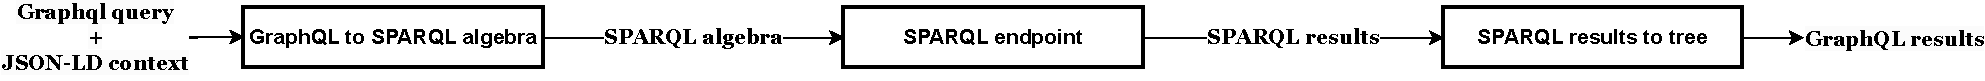
\includegraphics[width=0.80\linewidth]{images/graphql_overview.drawio.pdf}
  \caption{An overview of the flow process in GraphQL-LD}
  \label{fig:8}
\end{figure}

GraphQL-LD is predicate-oriented. This means that it focuses on querying the relationships between the subject and object~\cite{Werbrouck2019a}. This imposes a problem for implementing subject-based queries when we want to query for a specific class. An example for this would be querying for an item that is of type chemical element. To overcome this problem we would need a workaround. However, this makes the query complicated to write. In the next chapter where we implement querying Wikidata using GraphQL-LD, we discuss three workarounds that can used when we want to implement subject-based queries. 

Since GraphQL-LD is schema-less, it not possible to perform introspection\footnote{https://graphql.org/learn/introspection/} -  querying a GraphQL schema for information about the supported queries - since the user is not aware of the data's schema~\cite{Gleim2020}. However, this is not necessary since all exposed Linked Data can be queried with GraphQL-LD~\cite{Werbrouck2019a}. When writing queries, GraphQL-LD users would need to have a good understanding of the data scheme of the queried RDF data.  


\section{HyperGraphQL}

HyperGraphQL is open source GraphQL interface for querying Linked Data on the Web. It is developed and maintained by Semantics Integration Ltd. The project is written in Java, with the initial release being in 2018. At the time of this writing, the latest version, 3.0.1, was released in 2021.

HyperGraphQL is designed to support federated querying over multiple RDF stores via a single GraphQL query interface~\cite{Taelman2019}. Federated queries refer to querying multiple data sources and combining the data. This enriches the results with interesting information as the data is obtained from various sources rather than just one. However, federated querying is challenging. Retrieving and combining data from different services requires deep understanding of the involved datasets, and different configuration parameters such as authentication need to be considered. 

A service need to be set up that acts as an intermediary server between the client side, where the GraphQL query is written, and the RDF datastore, from where Linked Data is fetched~\cite{Taelman2018}. We can create multiple instances of HyperGraphQL where each instance can query one or more RDF sources, depending on the type of Linked Data services selected. In the next section we discuss these services in detail. To set up a HyperGraphQL instance two input files need to be provided - a configuration JSON file and an annotated GraphQL schema.

\subsection{Configuration File}
\label{subsec:configuration}

The configuration file contains the specifications of the RDF services from there data needs to be fetched. It includes the name of the instance, path of the GraphQL schema, HTTP settings of the instance and the specifications of the Linked Data services needed to fetch data. HyperGraphQL currently offers three types of Linked Data services: \texttt{SPARQLEndpointService}, \texttt{LocalModeSPARQLService} and \texttt{HGraphQLService}. 

The \texttt{SPARQLEndpointService} refers to the SPARQL endpoint service where data is fetched from remote RDF sources, like Wikidata and DBpedia. \texttt{LocalModeSPARQLService} allows to fetch data from RDF files that exists on the local system or in a remote location. These files contain data stored as RDF triples and follow the RDF serialization format of RDF/XML, Turle or N-Triples. Lastly, the \texttt{HGraphQLService} allows to query data from other HyperGraphQL instances running on a server.

Listing~\ref{lst:15} shows a configuration file for fetching data from \textit{example.org} through the \texttt{SPARQLEndpointService}.

\begin{minipage}{\linewidth}
\begin{lstlisting}[label=lst:15, caption={An example configuration file}, language=GraphQLException3]
{
  "name":"example-hgql",
  "schema":"schema/schema_example.graphql",
  "server":{
    "port":8081,
    "graphql":"/graphql",
    "graphiql":"/graphiql"
  },
  "services":[
    {
      "id":"example-sparql",
      "type":"SPARQLEndpointService",
      "url":"http://example.org/sparql/",
      "graph":"",
      "user":"",
      "password":""
    }
  ]
}
\end{lstlisting}
\end{minipage}

\subsection{Annotated Schema}
\label{subsec:annotated-schema}
HyperGraphQL works with a GraphQL schema that needs to be defined to set up an instance. This is different from GraphQL-LD, where no schema is required. A schema gives control to the data that be queried. The user can only fetch data for the types and queries defined in the GraphQL schema~\cite{Gleim2020}.

The schema contains a designated type called \texttt{\_Context}. This contains the annotations that encode the mappings from every type and field in the schema to the corresponding IRI in the RDF source. The IRI should be unique and will be used to fetch data from the source. 

Each type and field in the schema is annotated with GraphQL directives that tell the instance about the service from where data for the type and filed should be fetched. These are essentially pointers or service ids that correspond to the RDF services defined in the configuration file.

Only the types annotated with a service id can be queried. Non-annotated typed will not be queryable. However, all fields need be annotated with a service id. For every annotated type, two query fields are automatically exposed - \textit{TypeName\_GET}, parametrized with the \texttt{limit:Int} and \texttt{offset:Int} argument, and \textit{TypeName\_GET\_BY\_ID}, parameterized with \texttt{uris:[String]} argument. Two additional fields are also introduced automatically for each type in the schema - \texttt{\_id:String} field which returns the IRI of the resource and \texttt{\_type:String} field which returns the \textit{rdf:type} of the parent type of the resource in the schema. Moreover, every field in the schema with the value type String is provided with a \texttt{lang:String} argument by default. This allows the user to specify the language of the fetched literal. However, only one language can be specified.

Listing~\ref{lst:16} shows a GraphQL schema that can be used to query data from \textit{example.org}, using the above configuration file. The \texttt{id:"example-sparql"} in the \textit{@service} directory is the same as the id in the services block of the configuration file.


\begin{minipage}{\linewidth}
\begin{lstlisting}[label=lst:16, caption={An example schema}, language=GraphQL]
type __Context {
  ChemicalElement:    _@href(iri: "http://example.org/chemicalElement")
  name:               _@href(iri: "http://example.org/name")
  chemicalFormula:   _@href(iri: "http://example.org/chemicalFormula")
  boilingPoint:       _@href(iri: "http://example.org/boilingPoint")
}

type ChemicalElement @service(id:"example-sparql") {
  name: String @service(id:"example-sparql")
  chemicalFormula: String @service(id:"example-sparql")
  boilingPoint: String @service(id:"example-sparql")
}
\end{lstlisting}
\end{minipage}

Like GraphQL-LD, HyperGraphQL also converts GraphQL queries into SPARQL. However, unlike GraphQL-LD where the conversion takes place on the client side, in HyperGraphQL the conversion takes place on the server side, thereby decreasing the computation overhead on the client side. Also, the generated SPARQL queries are not necessarily part of the user interaction, and are not displayed. We discuss in the next chapter when we implement HyperGraphQL to query Wikidata, the method we used to observe the generated SPARQL queries whenever an instance is set up.

Listings~\ref{lst:17} and \ref{lst:18} show a GraphQL querly based on our annotated schema and the generated SPARQL query respectively.


\begin{minipage}{\linewidth}
\begin{lstlisting}[label=lst:17, caption={An example query in HyperGraphQL}, language=GraphQL]
{
  ChemicalElement_GET {
    name
    chemicalFormula
    boilingPoint
  }
}
\end{lstlisting}
\end{minipage}


\begin{minipage}{\linewidth}
\begin{lstlisting}[columns=fullflexible, label=lst:18, caption={The generated SPARQL query}, language=SPARQL]
SELECT * WHERE { 
  { 
    SELECT ?x_1 WHERE { 
      ?x_1 <http://www.w3.org/1999/02/22-rdf-syntax-ns#type> <http://example.org/chemicalElement> . 
	}  
  }  
  OPTIONAL { 
    ?x_1 <http://example.org/name> ?x_1_1 . 
  }  
  OPTIONAL { 
    ?x_1 <http://example.org/chemicalFormula> ?x_1_2 . 
  }  
  OPTIONAL { 
    ?x_1 <http://example.org/boilingPoint> ?x_1_3 . 
  }  
}
\end{lstlisting}
\end{minipage}

We discussed in the previous section we discussed that in GraphQL-LD implementation, the result set is empty if any of the fields does not fetch a result (if the \texttt{@optional} directive is not given to the field in the GraphQL query). With HyperGraphQL this is relaxed since the fields are translated into \texttt{OPTIONAL} SPARQL triple patterns.

Once the instance runs on the local server, a \textit{graphiQL}\footnote{https://github.com/graphql/graphiql} interface is created. This is a graphical user interface where the user can write GraphQL queries and send them to the HyperGraphQL instance running on the local server. The instance queries the RDF data and returns a response in JSON-LD enhanced with JSON-LD context. Other RDF serialization formats are also supported for the returned response like \textit{json+rdf+xml} and \textit{json+turtle}. 